% -----------------------------------------------
% Vlastní text práce (kapitoly práce)
% -----------------------------------------------

% -----------------------------------------------
\chapter{Calibration UV optical source}
% -----------------------------------------------
Blah blah we need it.
% -----------------------------------------------
\section{Karlsruhe UV source}
% -----------------------------------------------


 \begin{figure}[H]
 \centering
 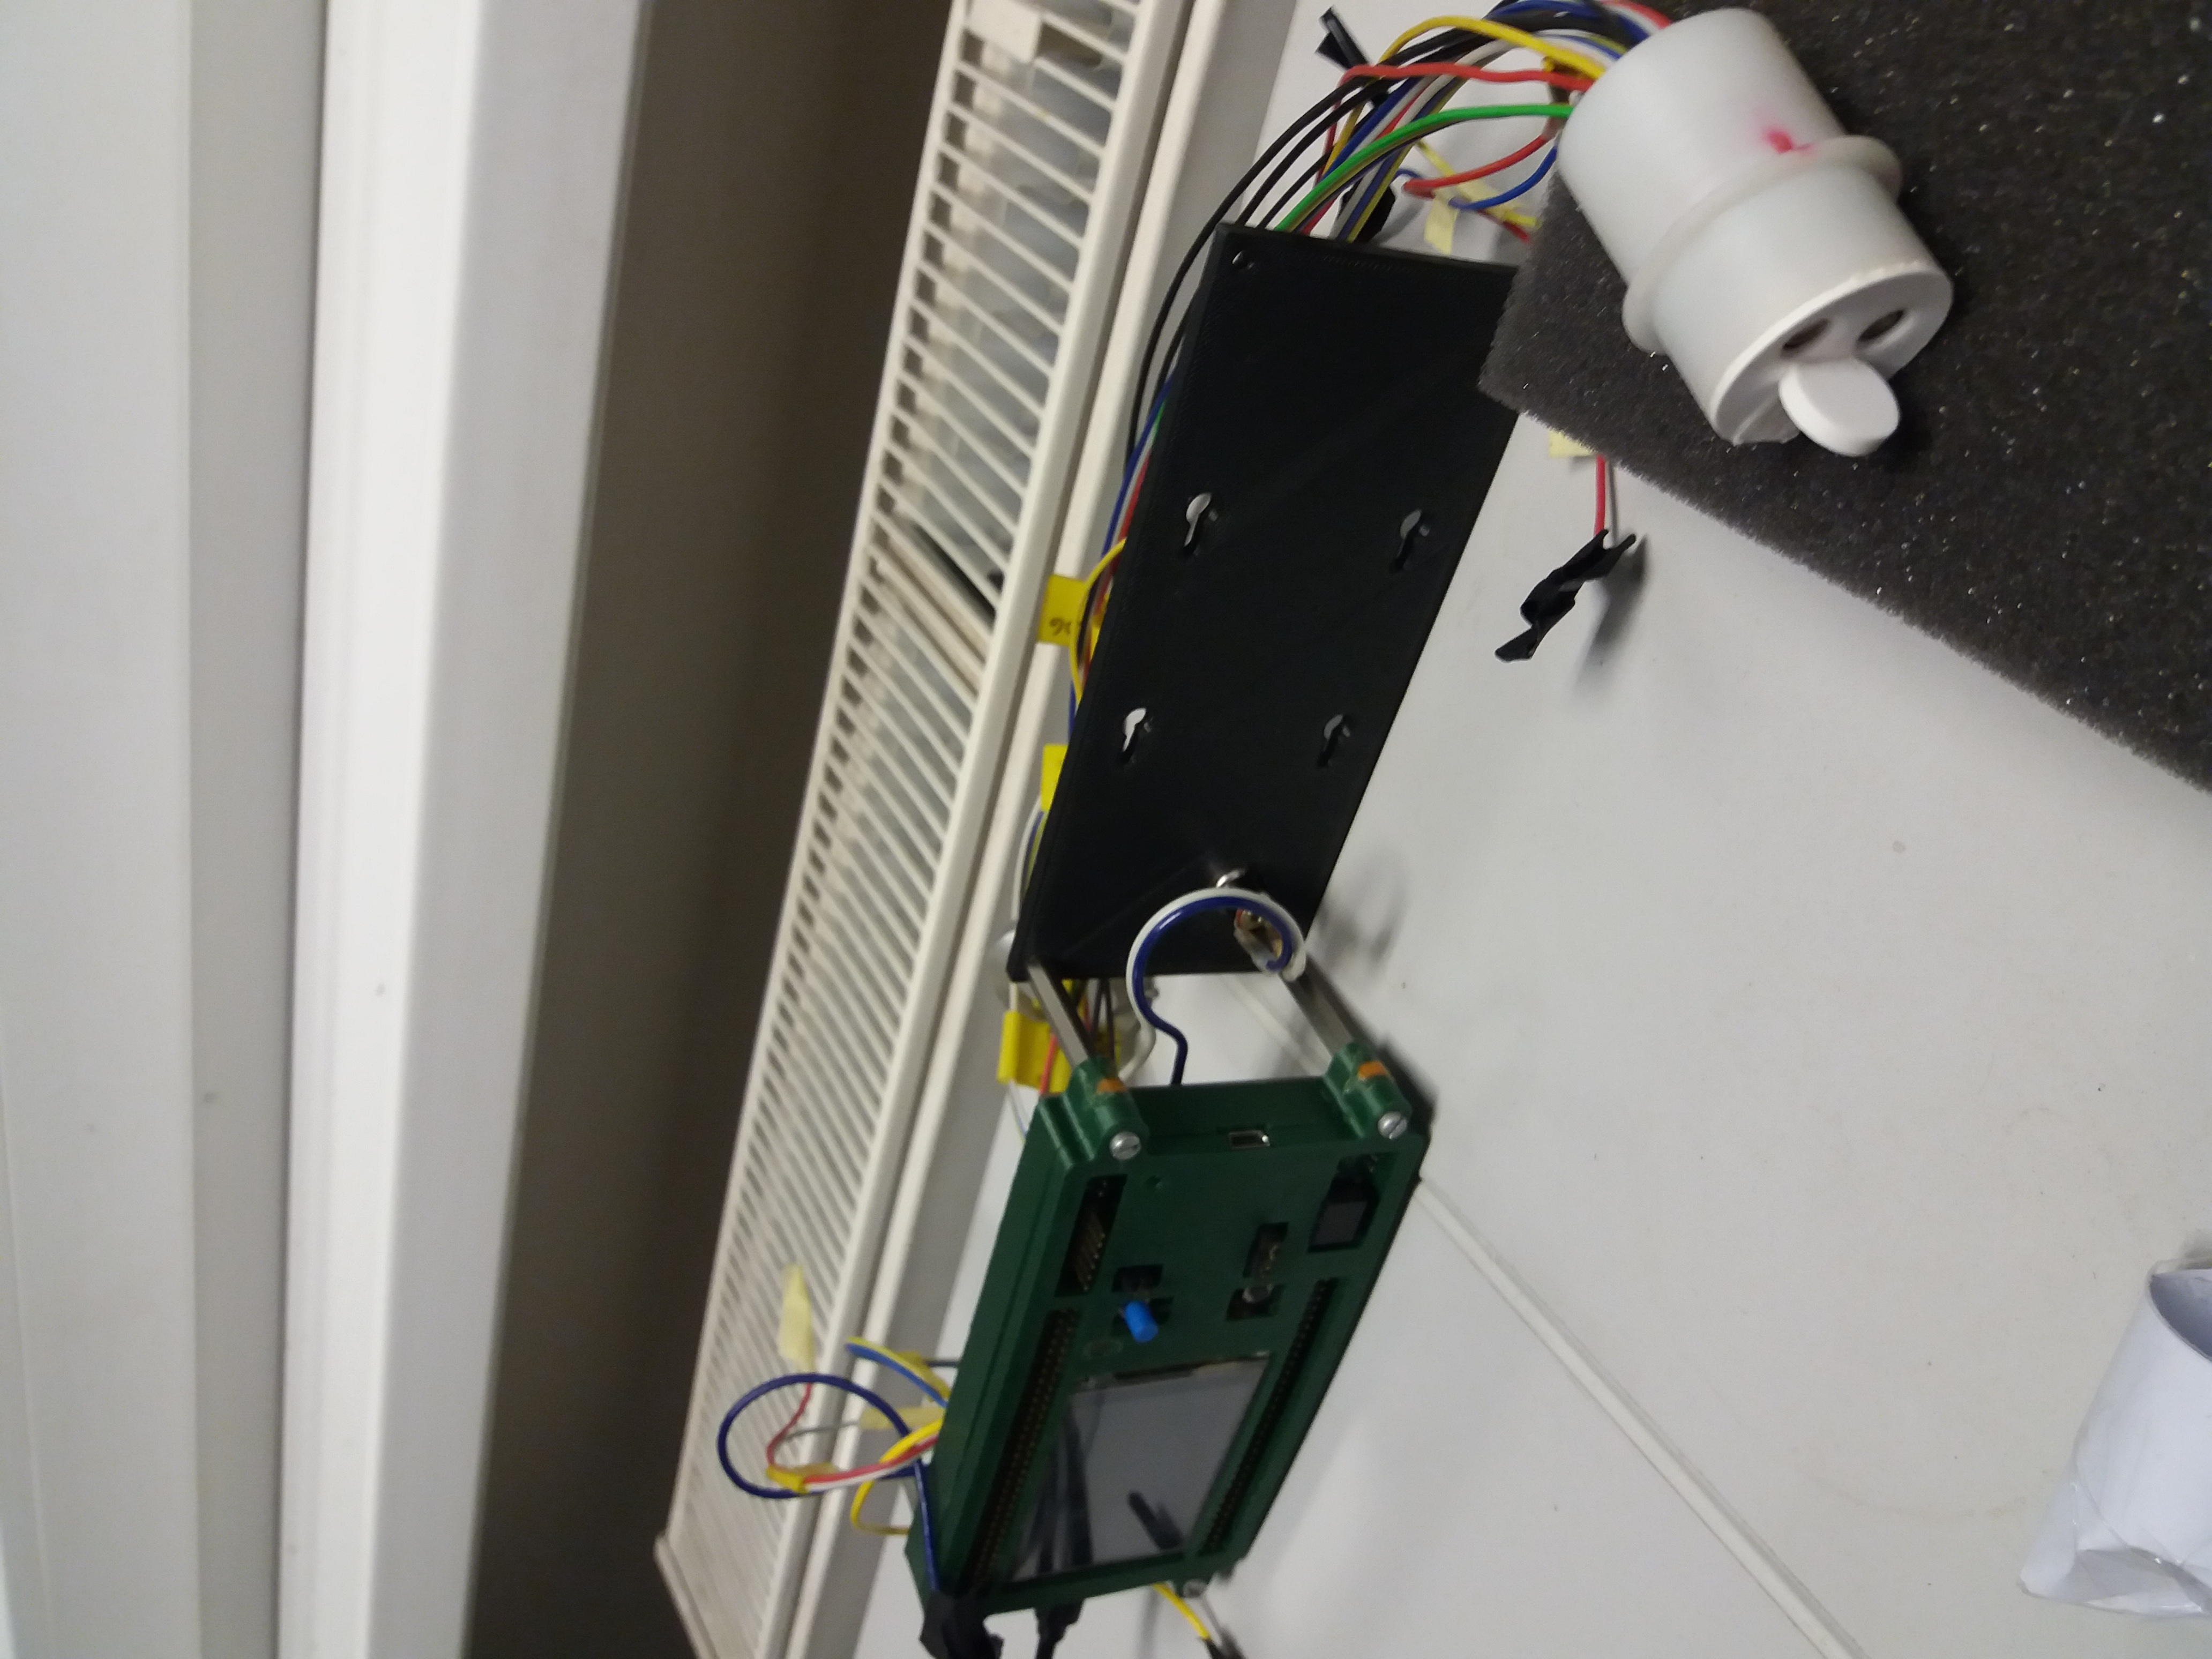
\includegraphics[scale=0.09, angle = 270, origin = c]{./pictures/KarlsRuhe}
 \caption{UV source conctructed according to KIT's template.}
 \label{UVsource}
\end{figure}


Our main task was to test this UV source's longtime stability and develop possible fixes and upgrades.

% -----------------------------------------------

\section{Testing and measurement of UV source}
% -----------------------------------------------
For calibration UV source, the longtime stability of optical power and pulse geometry is very important. Because there were no specialized apparatus for this measurement, we had to built and program one by ourselves.
\subsection{Measuring apparatus}
For measuring the optical power we use PM16 power meter (PM) and for determining the pulse geometry we use XP2262 PMT with signal output connected to 2-channel PicoScope 2205A MSO usb osciloscope. XP2262 PMT is held on $U \approx -680$ V by HV voltage source.
\par
We also use DS18B20 thermometer for PMT temperature monitoring and keysight 34461a multimeter for checking voltages.

\par
The PMT, power meter and the optical head of UV source are mounted in the IS's ports. The IS stops the unwanted external light and distributes the optical power to PMT and power meter. 
\par
The entire apparatus is driven by Raspberry Pi (RPi). The RPi takes care of data acquisiton and could be used to set the parameters of the UV source. It could be easilly accessed over internet for data download or for user to control the experiment.
\par
Osciloscope was programmed in C language according to its programmer's manual \ref{PicoScope}. It is capable of 2ns sampling which is enough to capture rising edges of the pulses. The RPi sets basic parameters (DC coupling, range etc.) and then activates osciloscope's trigger (rising edge). After sampling, RPi receives all samples from osciloscope's memory.

\par
Main component (IS,PW, PMT with HV source, UV source) are situated in protection box to prevent unwanted manipulations and touching the HV parts.The apparatus could be seen on fig. \ref{aparature1} and \ref{aparature2}.

\begin{figure}[H]
 \centering
 \includegraphics[width=150mm]{./pictures/aprature1b}
 \caption{Measuring apparatus.}
 \label{aparature1}
\end{figure}

\begin{figure}[H]
 \centering
 \includegraphics[scale = 0.09]{./pictures/aparature2b}
 \caption{PMT mounting and HV source.}
 \label{aparature2}
\end{figure}


\subsection{Data acquisition and analysis}
All the data are taken in specified interval (15 or 30 minutes). Two files are produced - osciloscope waveform file and a file with 30 samples of power meter, multimeter and a thermometer readings.
\par
The data from osciloscope contains the square pulses with noise (fig. \ref{pulse}). From them we need to extract the information of pulses height, slope and time of the rising edge.

 \begin{figure}[H]
 \centering
 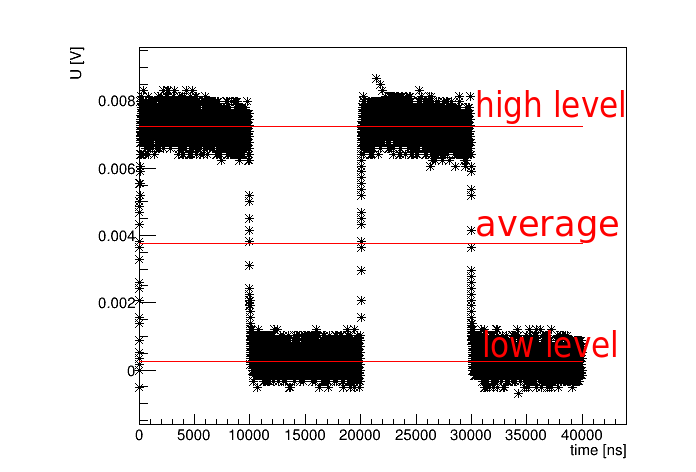
\includegraphics[scale=0.65]{./pictures/PMTPulse}
 \caption{Determining the basic pulse properties - average, low and high levels of signal.}
 \label{pulse}
\end{figure}

To determine the pulse height, we need to calculate the average value from all the samples at first. Then, we split the samples into two subgroups according to fact, whether they are higher or lower than the average. These subgroups are converted to histograms with fixed binning (around 5000 bins). These histograms are then fitted by gaussian. The means of these two fits determine two levels of the pulse - high ($U_\textrm{h}$) and low ($U_\textrm{l}$). The fig. \ref{pulse} shows the real pulse with levels determined by this method. The height of pulse is then simply calculated by substracting two levels: $U_\textrm{H} = U_\textrm{h} - U_\textrm{l}$.

\par
The properties the rising edge could be specified by two parameters, which we are able to extract from our data - time and the slope of the rising edge. We are able to calculate both of them if we identify the samples, which are taken at the time of the rising. These samples' values should be between 10 $\%$ and 90 $\%$ of the $U_{H}$. First, we need to detect the rising edge in waveform data sequence. However, the signal is very noisy and this could not be simply done by detecting the exceeding of the 10 $\%$ of the $U_{H}$ .To achieve that, we cycle through the waveform until we meet two conditions - the value is higher than average and the derivative is positive. Due to the noise, the derivative could not be calculated from two or three points, thus we use Savitzky–Golay polynom's derivative at chosen point: $y' = \frac{1}{12h}(y_{i-2} -8y_{i-1} + 8y_{i+1} - y_{i+2}) $. However we care only of positive/negative sign, so $\frac{1}{12h}$, where $h$ is the small step, is no use for us. When these two conditions are met at some point, the program cycles back from the point through the waveform until reaches $10\%$ level, and then beginning at the same point, which met the conditions, cycles up to reaching $90\%$ level. All the samples traversed by this way are considered as samples of the rising edge. The rising time is calculated simply by multipling the number of these samples by osciloscope's sample time (2 ns). The slope is calculated from linear fit of these samples (fig. \ref{linfit}).  


 \begin{figure}[H]
 \centering
 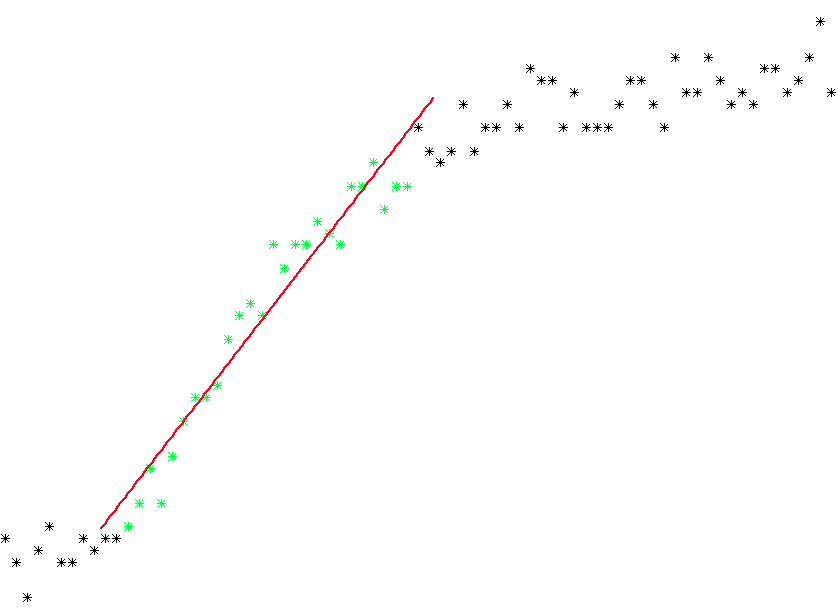
\includegraphics[scale=0.65]{./pictures/linFit}
 \caption{Linear fit of rising edge points (marked as green).}
 \label{linfit}
\end{figure}


\subsection{Results}

\section{UV LED diode aging}

%------------------------------------------------
\section{Optical feedback - potential fix}
% -----------------------------------------------
One way to handle the aging process of UV LED diodes is to monitor the power and according to the changes set the diode current. 


%------------------------------------------------

\section{Modified UV source for drone mounting}
% -----------------------------------------------



% -----------------------------------------------
% %%%%%%%%%%%%%%%%%%%%%%%% End of file %%%%%%%%%%%%%%%%%%%%%%%%
